\documentclass[12pt,twoside]{article}

\newcommand{\reporttitle}{495 Advanced Statistical Machine Learning and Pattern Recognition}
\newcommand{\reportauthor}{Thomas Teh}
\newcommand{\reporttype}{Notes}
\newcommand{\cid}{0124 3008}

% include files that load packages and define macros
%%%%%%%%%%%%%%%%%%%%%%%%%%%%%%%%%%%%%%%%%
% University Assignment Title Page 
% LaTeX Template
% Version 1.0 (27/12/12)
%
% This template has been downloaded from:
% http://www.LaTeXTemplates.com
%
% Original author:
% WikiBooks (http://en.wikibooks.org/wiki/LaTeX/Title_Creation)
%
% License:
% CC BY-NC-SA 3.0 (http://creativecommons.org/licenses/by-nc-sa/3.0/)
% 
% Instructions for using this template:
% This title page is capable of being compiled as is. This is not useful for 
% including it in another document. To do this, you have two options: 
%
% 1) Copy/paste everything between \begin{document} and \end{document} 
% starting at \begin{titlepage} and paste this into another LaTeX file where you 
% want your title page.
% OR
% 2) Remove everything outside the \begin{titlepage} and \end{titlepage} and 
% move this file to the same directory as the LaTeX file you wish to add it to. 
% Then add \input{./title_page_1.tex} to your LaTeX file where you want your
% title page.
%
%----------------------------------------------------------------------------------------
%	PACKAGES AND OTHER DOCUMENT CONFIGURATIONS
%----------------------------------------------------------------------------------------
\usepackage{ifxetex}
\usepackage{textpos}
\usepackage{natbib}
%\usepackage{breqn}
\usepackage{kpfonts}
\usepackage[a4paper,hmargin=2.8cm,vmargin=2.0cm,includeheadfoot]{geometry}
\usepackage{ifxetex}
\usepackage{stackengine}
\usepackage{tabularx,longtable,multirow,subfigure,caption}%hangcaption
\usepackage{fncylab} %formatting of labels
\usepackage{fancyhdr}
\usepackage{color}
\usepackage[tight,ugly]{units}
\usepackage{url}
\usepackage{float}
\usepackage[english]{babel}
\usepackage{amsmath}
\usepackage{graphicx}
\usepackage[colorinlistoftodos]{todonotes}
\usepackage{dsfont}
\usepackage{epstopdf} % automatically replace .eps with .pdf in graphics
\usepackage{natbib}
\usepackage{backref}
\usepackage{array}
\usepackage{latexsym}
\usepackage{etoolbox}

\usepackage{enumerate} % for numbering with [a)] format 



\ifxetex
\usepackage{fontspec}
\setmainfont[Scale=.8]{OpenDyslexic-Regular}
\else
\usepackage[pdftex,pagebackref,hypertexnames=false,colorlinks]{hyperref} % provide links in pdf
\hypersetup{pdftitle={},
  pdfsubject={}, 
  pdfauthor={\reportauthor},
  pdfkeywords={}, 
  pdfstartview=FitH,
  pdfpagemode={UseOutlines},% None, FullScreen, UseOutlines
  bookmarksnumbered=true, bookmarksopen=true, colorlinks,
    citecolor=black,%
    filecolor=black,%
    linkcolor=black,%
    urlcolor=black}
\usepackage[all]{hypcap}
\fi

\usepackage{tcolorbox}

% various theorems
\usepackage{ntheorem}
\theoremstyle{break}
\newtheorem{lemma}{Lemma}
\newtheorem{theorem}{Theorem}
\newtheorem{remark}{Remark}
\newtheorem{definition}{Definition}
\newtheorem{proof}{Proof}

% example-environment
\newenvironment{example}[1][]
{ 
\vspace{4mm}
\noindent\makebox[\linewidth]{\rule{\hsize}{1.5pt}}
\textbf{Example #1}\\
}
{ 
\noindent\newline\makebox[\linewidth]{\rule{\hsize}{1.0pt}}
}



%\renewcommand{\rmdefault}{pplx} % Palatino
% \renewcommand{\rmdefault}{put} % Utopia

\ifxetex
\else
\renewcommand*{\rmdefault}{bch} % Charter
\renewcommand*{\ttdefault}{cmtt} % Computer Modern Typewriter
%\renewcommand*{\rmdefault}{phv} % Helvetica
%\renewcommand*{\rmdefault}{iwona} % Avant Garde
\fi

\setlength{\parindent}{0em}  % indentation of paragraph

\setlength{\headheight}{14.5pt}
\pagestyle{fancy}
\fancyfoot[ER,OL]{\thepage}%Page no. in the left on
                                %odd pages and on right on even pages
\fancyfoot[OC,EC]{\sffamily }
\renewcommand{\headrulewidth}{0.1pt}
\renewcommand{\footrulewidth}{0.1pt}
\captionsetup{margin=10pt,font=small,labelfont=bf}


%--- chapter heading

\def\@makechapterhead#1{%
  \vspace*{10\p@}%
  {\parindent \z@ \raggedright %\sffamily
        %{\Large \MakeUppercase{\@chapapp} \space \thechapter}
        %\\
        %\hrulefill
        %\par\nobreak
        %\vskip 10\p@
    \interlinepenalty\@M
    \Huge \bfseries 
    \thechapter \space\space #1\par\nobreak
    \vskip 30\p@
  }}

%---chapter heading for \chapter*  
\def\@makeschapterhead#1{%
  \vspace*{10\p@}%
  {\parindent \z@ \raggedright
    \sffamily
    \interlinepenalty\@M
    \Huge \bfseries  
    #1\par\nobreak
    \vskip 30\p@
  }}
  



% %%%%%%%%%%%%% boxit
\def\Beginboxit
   {\par
    \vbox\bgroup
	   \hrule
	   \hbox\bgroup
		  \vrule \kern1.2pt %
		  \vbox\bgroup\kern1.2pt
   }

\def\Endboxit{%
			      \kern1.2pt
		       \egroup
		  \kern1.2pt\vrule
		\egroup
	   \hrule
	 \egroup
   }	

\newenvironment{boxit}{\Beginboxit}{\Endboxit}
\newenvironment{boxit*}{\Beginboxit\hbox to\hsize{}}{\Endboxit}



\allowdisplaybreaks

\makeatletter
\newcounter{elimination@steps}
\newcolumntype{R}[1]{>{\raggedleft\arraybackslash$}p{#1}<{$}}
\def\elimination@num@rights{}
\def\elimination@num@variables{}
\def\elimination@col@width{}
\newenvironment{elimination}[4][0]
{
    \setcounter{elimination@steps}{0}
    \def\elimination@num@rights{#1}
    \def\elimination@num@variables{#2}
    \def\elimination@col@width{#3}
    \renewcommand{\arraystretch}{#4}
    \start@align\@ne\st@rredtrue\m@ne
}
{
    \endalign
    \ignorespacesafterend
}
\newcommand{\eliminationstep}[2]
{
    \ifnum\value{elimination@steps}>0\leadsto\quad\fi
    \left[
        \ifnum\elimination@num@rights>0
            \begin{array}
            {@{}*{\elimination@num@variables}{R{\elimination@col@width}}
            |@{}*{\elimination@num@rights}{R{\elimination@col@width}}}
        \else
            \begin{array}
            {@{}*{\elimination@num@variables}{R{\elimination@col@width}}}
        \fi
            #1
        \end{array}
    \right]
    & 
    \begin{array}{l}
        #2
    \end{array}
    &%                                    moved second & here
    \addtocounter{elimination@steps}{1}
}
\makeatother

%% Fast macro for column vectors
\makeatletter  
\def\colvec#1{\expandafter\colvec@i#1,,,,,,,,,\@nil}
\def\colvec@i#1,#2,#3,#4,#5,#6,#7,#8,#9\@nil{% 
  \ifx$#2$ \begin{bmatrix}#1\end{bmatrix} \else
    \ifx$#3$ \begin{bmatrix}#1\\#2\end{bmatrix} \else
      \ifx$#4$ \begin{bmatrix}#1\\#2\\#3\end{bmatrix}\else
        \ifx$#5$ \begin{bmatrix}#1\\#2\\#3\\#4\end{bmatrix}\else
          \ifx$#6$ \begin{bmatrix}#1\\#2\\#3\\#4\\#5\end{bmatrix}\else
            \ifx$#7$ \begin{bmatrix}#1\\#2\\#3\\#4\\#5\\#6\end{bmatrix}\else
              \ifx$#8$ \begin{bmatrix}#1\\#2\\#3\\#4\\#5\\#6\\#7\end{bmatrix}\else
                 \PackageError{Column Vector}{The vector you tried to write is too big, use bmatrix instead}{Try using the bmatrix environment}
              \fi
            \fi
          \fi
        \fi
      \fi
    \fi
  \fi 
}  
\makeatother

\robustify{\colvec}

%%% Local Variables: 
%%% mode: latex
%%% TeX-master: "notes"
%%% End: 
 % various packages needed for maths etc.
% quick way of adding a figure
\newcommand{\fig}[3]{
 \begin{center}
 \scalebox{#3}{\includegraphics[#2]{#1}}
 \end{center}
}

%\newcommand*{\point}[1]{\vec{\mkern0mu#1}}
\newcommand{\ci}[0]{\perp\!\!\!\!\!\perp} % conditional independence
\newcommand{\point}[1]{{#1}} % points 
\renewcommand{\vec}[1]{{\boldsymbol{{#1}}}} % vector
\newcommand{\mat}[1]{{\boldsymbol{{#1}}}} % matrix
\newcommand{\R}[0]{\mathds{R}} % real numbers
\newcommand{\Z}[0]{\mathds{Z}} % integers
\newcommand{\N}[0]{\mathds{N}} % natural numbers
\newcommand{\nat}[0]{\mathds{N}} % natural numbers
\newcommand{\Q}[0]{\mathds{Q}} % rational numbers
\ifxetex
\newcommand{\C}[0]{\mathds{C}} % complex numbers
\else
\newcommand{\C}[0]{\mathds{C}} % complex numbers
\fi
\newcommand{\tr}[0]{\text{tr}} % trace
\renewcommand{\d}[0]{\mathrm{d}} % total derivative
\newcommand{\inv}{^{-1}} % inverse
\newcommand{\id}{\mathrm{id}} % identity mapping
\renewcommand{\dim}{\mathrm{dim}} % dimension
\newcommand{\rank}[0]{\mathrm{rk}} % rank
\newcommand{\determ}[1]{\mathrm{det}(#1)} % determinant
\newcommand{\scp}[2]{\langle #1 , #2 \rangle}
\newcommand{\kernel}[0]{\mathrm{ker}} % kernel/nullspace
\newcommand{\img}[0]{\mathrm{Im}} % image
\newcommand{\idx}[1]{{(#1)}}
\DeclareMathOperator*{\diag}{diag}
\newcommand{\E}{\mathds{E}} % expectation
\newcommand{\var}{\mathds{V}} % variance
\newcommand{\gauss}[2]{\mathcal{N}\big(#1,\,#2\big)} % gaussian distribution N(.,.)
\newcommand{\gaussx}[3]{\mathcal{N}\big(#1\,|\,#2,\,#3\big)} % gaussian distribution N(.|.,.)
\newcommand{\gaussBig}[2]{\mathcal{N}\left(#1,\,#2\right)} % see above, but with brackets that adjust to the height of the arguments
\newcommand{\gaussxBig}[3]{\mathcal{N}\left(#1\,|\,#2,\,#3\right)} % see above, but with brackets that adjust to the height of the arguments
\DeclareMathOperator{\cov}{Cov} % covariance (matrix) 
\ifxetex
\renewcommand{\T}[0]{^\top} % transpose
\else
\newcommand{\T}[0]{^\top}
\fi
% matrix determinant
\newcommand{\matdet}[1]{
\left|
\begin{matrix}
#1
\end{matrix}
\right|
}



%%% various color definitions
\definecolor{darkgreen}{rgb}{0,0.6,0}

\newcommand{\blue}[1]{{\color{blue}#1}}
\newcommand{\red}[1]{{\color{red}#1}}
\newcommand{\green}[1]{{\color{darkgreen}#1}}
\newcommand{\orange}[1]{{\color{orange}#1}}
\newcommand{\magenta}[1]{{\color{magenta}#1}}
\newcommand{\cyan}[1]{{\color{cyan}#1}}


% redefine emph
\renewcommand{\emph}[1]{\blue{\bf{#1}}}

% place a colored box around a character
\gdef\colchar#1#2{%
  \tikz[baseline]{%
  \node[anchor=base,inner sep=2pt,outer sep=0pt,fill = #2!20] {#1};
    }%
}%
 % short-hand notation and macros


%%%%%%%%%%%%%%%%%%%%%%%%%%%%

\begin{document}
% front page
% Last modification: 2016-09-29 (Marc Deisenroth)
\begin{titlepage}

\newcommand{\HRule}{\rule{\linewidth}{0.5mm}} % Defines a new command for the horizontal lines, change thickness here


%----------------------------------------------------------------------------------------
%	LOGO SECTION
%----------------------------------------------------------------------------------------


\includegraphics[width = 4cm]{./figures/imperial}\\[0.5cm] 

\begin{center} % Center remainder of the page

%----------------------------------------------------------------------------------------
%	HEADING SECTIONS
%----------------------------------------------------------------------------------------
\textsc{\LARGE \reporttype}\\[1.5cm] 
\textsc{\Large Imperial College London}\\[0.5cm] 
\textsc{\large Department of Computing}\\[0.5cm] 
%----------------------------------------------------------------------------------------
%	TITLE SECTION
%----------------------------------------------------------------------------------------

\HRule \\[0.4cm]
{ \huge \bfseries \reporttitle}\\ % Title of your document
\HRule \\[1.5cm]
\end{center}
%----------------------------------------------------------------------------------------
%	AUTHOR SECTION
%----------------------------------------------------------------------------------------

%\begin{minipage}{0.4\hsize}
\begin{flushleft} \large
\textit{Author:}\\
\reportauthor~(CID: \cid) % Your name
\end{flushleft}
\vspace{2cm}
\makeatletter
Date: \@date 

\vfill % Fill the rest of the page with whitespace



\makeatother


\end{titlepage}




%%%%%%%%%%%%%%%%%%%%%%%%%%%% Main document
\section{Expectation Maximization}

\subsection{General Approach for Expectation Maximization}
\subsubsection{Notes}
\begin{enumerate}
\item The goal of the Expectation-Maximization is to find maximum likelihood solutions for models having latent variables
\item The general concept is that since our knowledge of the latent variables in $\vec{Z}$ is given by the posterior distribution $p(\vec{Z}\vert \vec{Z}, \vec{\theta})$, we use the expectation of the latent variables instead of the actual values.
\item EM algorithm can be used to find MAP solutions models in which a prior is defined over the parameters.
\end{enumerate}

\subsubsection{Algorithm}
Given a joint distribution $p(\vec{X}, \vec{Z}\vert \vec{\theta})$ over observed variables $\vec{X}$ and latent variables $\vec{Z}$, governed by parameter $\vec{\theta}$ the goal is to maximize the likelihood function $p(\vec{X}\vert \vec{\theta})$ w.r.t $\vec{\theta}$.
\begin{enumerate}
\item Choose an initial for the parameters $\vec{\theta}^{old}$.
\item E Step: Evaluate $p(\vec{Z} \vert \vec{X}, \vec{\theta}^{old})$
\item M Step: Evaluate $\vec{\theta}^{new}$ given by
\begin{align*}
\vec{\theta}^{new}& = \text{arg} \max_{\vec{\theta}} \mathcal{Q}(\vec{\theta},\vec{\theta}^{old})
\end{align*}
where
\begin{align*}
\mathcal{Q}(\vec{\theta},\vec{\theta}^{old})& = \sum_{\vec{z}}p(\vec{Z}\vert \vec{X}, \vec{\theta}^{old})\ln p(\vec{X}, \vec{Z} \vert \vec{\theta})
\end{align*}
\item Check for convergence of either the log-likelihood or the parameter values. If convergence is not satisfied
\begin{align*}
\vec{\theta}^{old} \leftarrow \vec{\theta}^{new}
\end{align*}
and return to step 2
\end{enumerate}


\subsection{Gaussian Mixture Models}
The Gaussian mixture distribution can be written as a linear superposition of Gaussians
\begin{align*}
p(\vec{x}) &= \sum_{k=1}^K \pi_k \mathcal{N}(\vec{x}\vert \vec{\mu}_k, \vec{\Sigma}_k)
\end{align*}

\begin{figure}[H]
\begin{center}
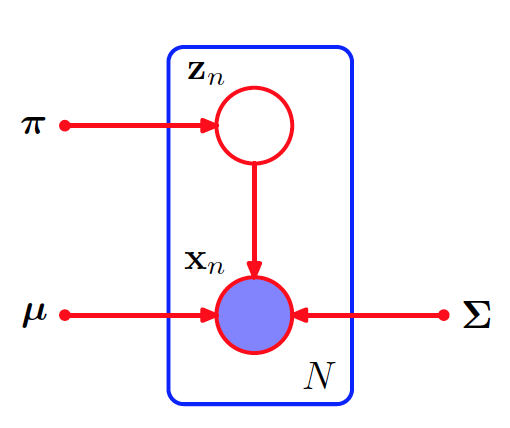
\includegraphics[width = 0.4\hsize]{./figures/GMM.png} % this includes the figure and specifies that it should span 0.7 times the horizontal size of the 
\caption{Gaussian Mixture Model.} % caption of the figure
\label{fig:GMM} % a label. When we refer to this label from the text, the figure number is included automatically
\end{center}
\end{figure}


\subsubsection{Formulation of the Gaussian Mixture Models}
Let $\vec{z}$ be a $K$-dimensional binary random variable with 1-of-$K$ representation.
\begin{align*}
p(z_k=1) = \pi_k 	&\Rightarrow p(\vec{z})=\prod_{i=1}^K \pi_k^{z_k}
\end{align*}

Conditional probability of $\vec{x}$ given a particular value for latent variable $\vec{z}$:
\begin{align*}
p(\vec{x}\vert \vec{z}) = \prod_{k=1}^K \mathcal{N}(\vec{x}\vert \vec{\mu}_k, \vec{\Sigma}_k)^{z_k}
\end{align*}

Using Bayes theorem and marginalize the latent variable $\vec{z}$
\begin{align*}
p(\vec{x}) =\sum_{\vec{z}}p(\vec{z})p(\vec{x}\vert \vec{z}) = \sum_{k=1}^K \pi_k\mathcal{N}(\vec{x}\vert \vec{\mu}_k, \vec{\Sigma}_k)
\end{align*}

Similarly, the posterior probability of $\vec{z}$ is given by
\begin{align*}
\gamma (z_k) = \frac{p(\vec{x}\vert \vec{z})p(\vec{z})}{p(\vec{x})} = \frac{\pi_k \mathcal{N}(\vec{x}\vert \vec{\mu}_k, \vec{\Sigma}_k) }{\sum_{j=1}^K \pi_j\mathcal{N}(\vec{x}\vert \vec{\mu}_j, \vec{\Sigma}_j)}
\end{align*}

\subsubsection{Maximum Likelihood}
The log-likelihood function is given by
\begin{align*}
\ln p(\vec{X} \vert \vec{\pi}, \vec{\mu}, \vec{\Sigma})&=\sum_{n=1}^N \ln\left(\sum_{k=1}^K \pi_k\mathcal{N}(\vec{x}\vert \vec{\mu}_k, \vec{\Sigma}_k)\right)
\end{align*}

The maximum likelihood method will yield the following:
\begin{align*}
\vec{\mu}_k & = \frac{\sum_{n=1}^N \gamma(z_{nk})\vec{x}_n}{\sum_{n=1}^N \gamma(z_{nk})}\\
\vec{\Sigma}_k& = \frac{\sum_{n=1}^N \gamma(z_{nk})(\vec{x}_n-\vec{\mu}_k)(\vec{x}_n-\vec{\mu}_k)^\top}{\sum_{n=1}^N \gamma(z_{nk})}\\
\pi_k&= \frac{\sum_{n=1}^N \gamma(z_{nk})}{N}
\end{align*}

Issues with maximum likelihood:
\begin{enumerate}
\item Presence of singularities: When we have at least two components in the mixture, one of them can have a finite variance and assign finite probability to all the data points, while the other component can shrink onto one specific data point and therefore contribute to an ever increasing additive value to the log likelihood.
\item Identifiability: Solutions may not be unique, hence it may be hard to interpret the parameter values discovered by a model.
\item The log likelihood equation is difficult to optimize over.
\end{enumerate}


\subsubsection{Expectation Maximization Formulation}
Supposed that in addition to $\vec{X}$, we were also given the values of the latent variables $\vec{Z}$, the likelihood and the log likelihood function are given by
\begin{align*}
p(\vec{X}, \vec{Z}\vert \vec{\mu}, \vec{\Sigma}, \vec{\pi})& =\prod_{n=1}^{N}\prod_{k=1}^{K} \pi_k^{z_{nk}}\mathcal{N}(\vec{x}_n\vert \vec{\mu}_k, \vec{\Sigma}_k)^{z_{nk}}\\
\ln p(\vec{X}, \vec{Z}\vert \vec{\mu}, \vec{\Sigma}, \vec{\pi})& =\sum_{n=1}^{N}\sum_{k=1}^{K} z_{nk}\left(\ln \pi_k + \ln \mathcal{N}(\vec{x}_n\vert \vec{\mu}_k, \vec{\Sigma}_k\right)
\end{align*}

\begin{enumerate}
\item \textbf{Expectation Step}:

Taking the expectation on the log likelihood 
\begin{align*}
\mathbb{E}_{p(\vec{Z}\vert \vec{X}, \vec{\theta})}\left[\ln p(\vec{X}, \vec{Z}\vert \vec{\mu}, \vec{\Sigma}, \vec{\pi})\right]
& =\sum_{n=1}^{N}\sum_{k=1}^{K} \mathbb{E}_{p(\vec{Z}\vert \vec{X}, \vec{\theta})}[z_{nk}]\left(\ln \pi_k + \ln \mathcal{N}(\vec{x}_n\vert \vec{\mu}_k, \vec{\Sigma}_k\right)\\
& = G(\vec{\theta})
\end{align*}

\begin{align*}
p(\vec{Z}\vert \vec{X}, \vec{\theta})\propto &
\prod_{n=1}^N\prod_{k=1}^K [\pi_k\mathcal{N}(\vec{x}_n\vert \vec{\mu}_k, \vec{\Sigma}_k)]^{z_{nk}}
\end{align*}

\begin{align*}
\mathbb{E}_{p(\vec{Z}\vert \vec{X}, \vec{\theta})}[z_{nk}]
&= \frac{\sum_{z_{nk}}z_{nk}[\pi_k\mathcal{N}(\vec{x}_n\vert \vec{\mu}_k, \vec{\Sigma}_k)]^{z_{nk}} }{\sum_{j=1}^K \pi_j \mathcal{N}(\vec{x}_n \vert \vec{\mu}_j, \vec{\Sigma}_j)}\\
&= \frac{\pi_k \mathcal{N}(\vec{x}_n \vert \vec{\mu}_k, \vec{\Sigma}_k)}{\sum_{j=1}^K \pi_j \mathcal{N}(\vec{x}_n \vert \vec{\mu}_j, \vec{\Sigma}_j)}\\
&=\gamma({z_{nk}})
\end{align*}

\item \textbf{Maximization Step}:
By taking the derivative of $(\vec{\theta})$ w.r.t $\vec{\theta}$ and set them to $0$, the parameters can be found to be
\begin{align*}
\vec{\mu}_k & = \frac{\sum_{n=1}^N \gamma(z_{nk})\vec{x}_n}{\sum_{n=1}^N \gamma(z_{nk})}\\
\vec{\Sigma}_k& = \frac{\sum_{n=1}^N \gamma(z_{nk})(\vec{x}_n-\vec{\mu}_k)(\vec{x}_n-\vec{\mu}_k)^\top}{\sum_{n=1}^N \gamma(z_{nk})}\\
\pi_k&= \frac{\sum_{n=1}^N \gamma(z_{nk})}{N}
\end{align*}

\end{enumerate}

\subsubsection{Expectation Maximization Algorithm}
Given a Gaussian mixture model, the goal is to maximize the likelihood functions w.r.t to the parameters:
\begin{enumerate}
\item Initialize the means $\vec{\mu}_k$, covariances $\vec{\Sigma}_k$ and mixing coefficients $\pi_k$ and evaluate the initial of the log likelihood.
\item E Step: Evaluate the responsibilities using the current parameter values
\begin{align*}
\gamma (z_k) = \frac{p(\vec{x}\vert \vec{z})p(\vec{z})}{p(\vec{x})} = \frac{\pi_k \mathcal{N}(\vec{x}\vert \vec{\mu}_k, \vec{\Sigma}_k) }{\sum_{j=1}^K \pi_j\mathcal{N}(\vec{x}\vert \vec{\mu}_j, \vec{\Sigma}_j)}
\end{align*}
\item M Step: Re-estimate the parameters using the current responsibilities
\begin{align*}
\vec{\mu}_k^{new}&=\frac{1}{N_k}\sum_{n=1}^N \gamma(z_{nk})\vec{x}_n\\
\vec{\Sigma}_k^{new}&=\frac{1}{N_k}\sum_{n=1}^N \gamma(z_{nk})(\vec{x}_n-\vec{\mu}_k)(\vec{x}_n-\vec{\mu}_k)^\top\\
\pi_k^{new}&=\frac{N_k}{N}
\end{align*}
where
\begin{align*}
N_k & = \sum_{n=1}^N \gamma(z_{nk})
\end{align*}
\item Evaluate the log likelihood
\begin{align*}
\ln p(\vec{X} \vert \vec{\pi}, \vec{\mu}, \vec{\Sigma})&=\sum_{n=1}^N \ln\left(\sum_{k=1}^K \pi_k\mathcal{N}(\vec{x}\vert \vec{\mu}_k, \vec{\Sigma}_k)\right)
\end{align*}
and check for convergence of either parameter of the log likelihood. If the convergence criterion is not satisfied, return to step 2
\end{enumerate}


\subsection{Bernoulli Mixture Models}

\begin{align*}
p(\vec{x}\vert \vec{\mu}) & = \prod_{i=1}^D \mu_i^{x_i}(1-\mu_i)^{1-x_i}\\
\mathbb{E}[\vec{x}] & = \vec{\mu}\\
\mathbb{V}[\vec{x}] &= diag\lbrace \mu_i(1-\mu_i)\rbrace
\end{align*}

The mixture of the Bernoulli distributions is given by
\begin{align*}
p(\vec{x}\vert \vec{\mu}, \vec{\pi})&=\sum_{k=1}^K \pi_kp(\vec{x}\vert \vec{\mu}_k)\\
p(\vec{x}\vert \vec{\mu}_k) &= \prod^{D}_{i=1} \mu_{ki}^{x_i} (1- \mu_{ki}^{x_i})^{1-x_i}\\
\mathbb{E}[\vec{x}] & = \sum_{k=1}^K \pi_k\vec{\mu}_k\\
\mathbb{V}[\vec{x}] &= \sum_{k=1}^K \pi_k \left(\vec{\Sigma}_k + \vec{\mu}_k\vec{\mu}_k^\top\right) - \mathbb{E}[\vec{X}]\mathbb{E}[\vec{X}]^\top\\
\vec{\Sigma}_k & = diag\lbrace \mu_{ki}(1-\mu_{ki})\rbrace
\end{align*}

Let $\vec{z}$ be the one hot representation, we have
\begin{align*}
p(\vec{x} \vert \vec{z}, \vec{\mu}) &= \prod_{k=1}^K p(\vec{x}\vert \vec{\mu}_k)^{z_k}\\
p(\vec{z}\vert \vec{\pi}) &= \prod_{k=1}^K \pi_k^{z_k}
\end{align*}

The log likelihood function is given by
\begin{align*}
\ln p(\vec{X}, \vec{Z} \vert \vec{\mu}, \vec{\pi})&=\sum_{n=1}^N\sum_{k=1}^Kz_{nk}
\left\lbrace 
\ln \pi_k +\sum_{i=1}^D[x_{ni}\ln\mu_{ki}+(1-x_{ni})\ln(1-\mu_{ki})]
\right\rbrace
\end{align*}

The E step: we then take the expectation of the log likelihood above
\begin{align*}
\mathbb{E}_{\vec{Z}}[\ln p(\vec{X}, \vec{Z} \vert \vec{\mu}, \vec{\pi})]&=\sum_{n=1}^N\sum_{k=1}^K\gamma(z_{nk})
\left\lbrace 
\ln \pi_k +\sum_{i=1}^D[x_{ni}\ln\mu_{ki}+(1-x_{ni})\ln(1-\mu_{ki})]
\right\rbrace\\
&\\
\gamma(z_{nk})& = \frac{\sum_{z_{nk}} z_{nk}[\pi_kp(\vec{x}_n\vert \vec{\mu}_k)]^{z_{nk}} }{\sum_{z_{nj}}[\pi_jp(\vec{x}_n\vert \vec{\mu}_j)]^{z_{nj}}}
=\frac{\pi_kp(\vec{x}_n\vert \vec{\mu}_k)}{\sum_{j=1}^K \pi_jp(\vec{x)_n}\vert \vec{\mu}_j)}
\end{align*}

The M step: we then maximize the log likelihood wrt to the parameters
\begin{align*}
\vec{\mu}_k &=\frac{1}{N_k}\sum_{n=1}^N \gamma(z_{nk})\\
\pi_k&=\frac{N_k}{N}\\
N_k &= \sum_{n=1}^N \gamma(z_{nk})
\end{align*}

\subsection{Convergence of the EM Algorithm}

\begin{align*}
p(\vec{X} \vert \vec{\theta}) = \sum_{\vec{Z}} p(\vec{X},\vec{Z} \vert \vec{\theta}) &\Rightarrow \ln p(\vec{X} \vert \vec{\theta}) = \mathcal{L}(q, \vec{\theta}) + KL(q\parallel p)\\
\mathcal{L}(q, \vec{\theta})&=\sum_{\vec{Z}} q(\vec{Z})\ln \left[\frac{p(\vec{X}, \vec{Z}\vert \vec{\theta})}{q(\vec{Z})}\right]\\
 KL(q\parallel p)&=-\sum_{\vec{Z}} q(\vec{Z})\ln \left[\frac{p(\vec{Z}\vert \vec{X}, \vec{\theta})}{q(\vec{Z})}\right]
\end{align*}

In the E step, the lower bound $\mathcal{L}(q,\vec{\theta}^{old})$ is maximized with respect to $q(\vec{Z})$. The solution to this maximization problem can be done by setting $q(\vec{Z}) = p (\vec{Z}\vert \vec{X}, \vec{\theta}^{old})$ such that $KL(q\parallel p)=0$.\\

In the M step, the lower bound $\mathcal{L}(q,\vec{\theta}^{old})$ is maximized with respect to $\vec{\theta}$. However, the KL divergence will no longer be zero. Hence, the increase in the upper bound of the log likelihood function is greater than the increase in the lower bound.\\

By substituting $q(\vec{Z}) = p(\vec{Z}\vert\vec{X}, \vec{\theta}^{old})$, we get the lower bound to be the following after the E step:
\begin{align*}
\mathcal{L}(q,\vec{\theta}) & = \sum_{\vec{Z}}p(\vec{Z}\vert \vec{X}, \vec{\theta}^{old})\ln p(\vec{X},\vec{Z}\vert \vec{\theta}) - \sum_{\vec{Z}}p(\vec{Z}\vert \vec{X}, \vec{\theta}^{old})\ln p(\vec{Z} \vert \vec{X}, \vec{\theta}^{old})\\
&= \mathcal{Q}(\vec{\theta},\vec{\theta}^{old} ) + const 
\end{align*}


\newpage

\section{Probabilistic PCA}

\begin{align*}
\vec{x} &= \vec{Wy} + \vec{\mu} + \vec{e}\\
\vec{e} & \sim \mathcal{N}(\vec{e}\vert \vec{0}, \sigma^2\vec{I})\\
\vec{y} & \sim \mathcal{N}(\vec{y}\vert \vec{0}, \vec{I})
\end{align*}


\begin{figure}[H]
\begin{center}
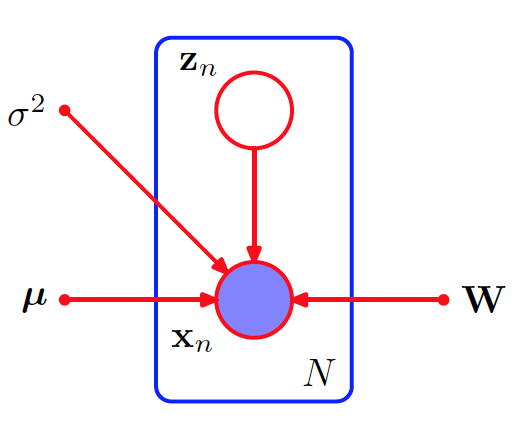
\includegraphics[width = 0.4\hsize]{./figures/PPCA.png} % this includes the figure and specifies that it should span 0.7 times the horizontal size of the 
\caption{Gaussian Mixture Model.} % caption of the figure
\label{fig:PPCA} % a label. When we refer to this label from the text, the figure number is included automatically
\end{center}
\end{figure}

\subsection{Maximum Likelihood}
\begin{enumerate}
\item We are interested in the distribution of $\vec{x}$ and the parameters $\vec{\theta}$. The marginal distribution of $\vec{x}$ can be obtained by integrating $\vec{y}$ out of the joint distribution.
\begin{align*}
p(\vec{x}_1,\dots, \vec{x}_N \vert \vec{\theta})
&=\int_{\vec{y_i}}p(\vec{x}_1,\dots, \vec{x}_N, \vec{y}_1,\dots, \vec{y}_N \vert \vec{\theta}) d\vec{y}_1\dots d\vec{y}_N\\
&= \int_{\vec{y_i}}\prod_{i=1}^N p(\vec{x}_i \vert \vec{y}_i,\vec{W}, \vec{\mu}, \sigma)p(\vec{y}_i)d\vec{y}_1\dots d\vec{y}_N\\
&= \prod_{i=1}^N\int_{\vec{y_i}} p(\vec{x}_i \vert \vec{y}_i,\vec{W}, \vec{\mu}, \sigma)p(\vec{y}_i)d\vec{y}_i
\end{align*}

\item The joint distribution can be obtained by applying Bayes' Rule.
\begin{align*}
p(\vec{x}_1,\dots, \vec{x}_N, \vec{y}_1,\dots, \vec{y}_N \vert \vec{\theta})
& = \prod_{i=1}^N p(\vec{x}_i \vert \vec{y}_i,\vec{W}, \vec{\mu}, \sigma)p(\vec{y}_i)\\
p(\vec{x}_i \vert \vec{y}_i,\vec{W}, \vec{\mu}, \sigma)p(\vec{y}_i) 
&= \left[(2\pi\sigma^2)^{-\frac{F}{2}} e^{-\frac{1}{2\sigma^2}(\vec{x_i}-\vec{\mu}-\vec{Wy_i})^\top(\vec{x_i}-\vec{\mu}-\vec{Wy_i})}\right]\left[(2\pi)^{-\frac{d}{2}}e^{-\frac{1}{2}\vec{y_i}^\top\vec{y_i}}\right]
\end{align*}

\item By collecting the $\vec{y}$ in the exponents, completing the squares and then applying the Woodbury identity (more details please refer to notes in 496):
\begin{align*}
p(\vec{x_i}\vert \vec{W}, \vec{\mu}, \sigma^2) & = \mathcal{N}(\vec{x_i}\vert \vec{\mu}, \vec{D} )\\
\vec{D}&=\vec{WW}^\top +\sigma^2\vec{I}\\
p(\vec{y_i}\vert \vec{x_i}, \vec{W}, \vec{\mu}, \sigma^2) & = \mathcal{N}(\vec{y_i} \vert \vec{M}^{-1}\vec{W}^\top(\vec{x_i}-\vec{\mu}), \sigma^2\vec{M}^{-1})\\
\vec{M}&=\sigma^2\vec{I} + \vec{W^\top W}
\end{align*}

\item  Maximizing the likelihood and solve for the parameters
\begin{align*}
\vec{S_t} & = \vec{U\Lambda U}^\top \text{ ($\vec{S_t}$ is the covariance matrix)}\\
\sigma^2 & = \frac{1}{F-d} \sum_{j= d+1}^F \lambda_j\\
\vec{W_d}&= \vec{U_d}(\vec{\Lambda} - \sigma^2\vec{I})^{\frac{1}{2}}\vec{V}^\top
\end{align*}

\item Hence we no longer have a projection but:
\begin{align*}
\mathbb{E}_{\vec{p(\vec{y_i}\vert \vec{x_i})}} [\vec{y_i}] & = \vec{M^{-1}W^\top (x_i - \mu)}\\
\vec{\widehat{x_i}}&= \vec{W}\mathbb{E}_{\vec{p(\vec{y_i}\vert \vec{x_i})}} [\vec{y_i}]  + \vec{\mu}
\end{align*}

\end{enumerate}


\subsection{EM PPCA}
\begin{enumerate}
\item Write the log likelihood of the joint distribution of the observed and latent variables
\begin{align*}
p(\vec{X,Y} \vert \vec{\theta}) &= \prod_{i=1}^N p(\vec{x_i \vert y_i, \theta})p(\vec{y_i})\\
\ln p(\vec{X,Y} \vert \vec{\theta}) &= \sum_{i=1}^N \left(\ln p(\vec{x_i \vert y_i, \theta})+ \ln p(\vec{y_i})\right)\\
\ln p(\vec{x_i} \vert \vec{y_i}, \vec{\theta}) &= -\frac{F}{2}\ln (2\pi\sigma^2) - \frac{1}{2\sigma^2}\vec{(x_i-Wy_i-\mu)^\top (x_i-Wy_i-\mu)}\\
\ln p(\vec{y_i})&= -\frac{1}{2}\vec{y_i^\top y_i}-\frac{D}{2}\ln 2\pi
\end{align*}

\item \textbf{E-Step:} Take the expectation on the log likelihood on the joint distribution:
\begin{align*}
\ln p(\vec{X,Y} \vert \vec{\theta}) &=\sum_{i=1}^N\left[-\frac{F}{2}\ln 2\pi\sigma^2 -\frac{1}{2\sigma^2}\vec{(x_i-Wy_i-\mu)^\top (x_i-Wy_i-\mu)} -\frac{1}{2}\vec{y_i^\top y_i}-\frac{D}{2}\ln 2\pi\right]
\end{align*}

Expanding the above and use the identities $\text{tr}\left[\vec{y_i^\top WW^\top y_i}\right]=\text{tr}\left[\vec{y_iy_i^\top WW^\top }\right]$
\begin{align*}
\mathbb{E}_{p(\vec{Y\vert X})} [\ln p(\vec{X,Y} \vert \vec{\theta})]
&=-\frac{NF}{2}\ln 2\pi\sigma^2 -\frac{ND}{2}\ln 2\pi\\
& -\sum_{i=1}^N\left\lbrace\frac{1}{2\sigma^2}\left[\vec{(x_i-\mu)^\top (x_i-\mu)} -2 (\vec{x_i}-\vec{\mu})^\top \vec{W} \mathbb{E}[\vec{y_i}] \right.\right.\\
&+\left.\left.\text{tr}\left[\mathbb{E}(\vec{y_i y_i^\top})\vec{W^\top W}\right]\right]+\frac{1}{2}\text{tr}\left[\mathbb{E}(\vec{y_i^\top y_i})\right]\right\rbrace
\end{align*}

We can obtain the moments of $\vec{y_i}$ from the earlier derivation of the PPCA
\begin{align*}
p(\vec{y_i}\vert \vec{x_i}, \vec{W}, \vec{\mu}, \sigma^2) & = \mathcal{N}(\vec{y_i} \vert \vec{M}^{-1}\vec{W}^\top(\vec{x_i}-\vec{\mu}), \sigma^2\vec{M}^{-1})\\
\vec{M}&=\sigma^2\vec{I} + \vec{W^\top W}\\
\mathbb{E}_{p(\vec{Y\vert X})}[\vec{y_i}]&=\vec{M}^{-1}\vec{W}^\top(\vec{x_i}-\vec{\mu})\\
\mathbb{E}_{p(\vec{Y\vert X})}[\vec{y_i y_i^\top}]&=\sigma^2\vec{M}^{-1} +\mathbb{E}[\vec{y_i}]\mathbb{E}[\vec{y_i}]^\top
\end{align*}

\item \textbf{M-Step:} Maximize the log likelihood
\begin{align*}
\vec{\mu}&= \frac{1}{N}\sum_{i=1}^N(\vec{x_i} - \vec{W}\mathbb{E}[\vec{y_i}])\\
\vec{W}&=\left[\sum_{i=1}^N (\vec{x_i} - \vec{\mu})\mathbb{E}[\vec{y_i}]^\top]\right]\left[\sum_{i=1}^N \mathbb{E}[\vec{y_iy_i}^\top]\right]^{-1}\\
\sigma^2&=\frac{1}{NF}\sum_{i=1}^N\left\lbrace \parallel \vec{x_i-\mu} \parallel^2 -2\mathbb{E}[\vec{y_i}]^\top\vec{W^\top (x_i-\mu)} +\text{tr}(\mathbb{E}[\vec{y_iy_i^\top}]\vec{W^\top W})\right\rbrace
\end{align*}


\item Advantages of EM PPCA:
\begin{itemize}
\item A complexity of $O(NFD)$ can be significantly smaller than $O(NF^2)$ (from the computation of the covariance)
\item The EM procedure can be extended to factor analysis model
\item EM allows us to deal with missing values
\end{itemize}

\end{enumerate}


\section{PPCA Mixture Model and Applications}

\begin{figure}[H]
\begin{center}
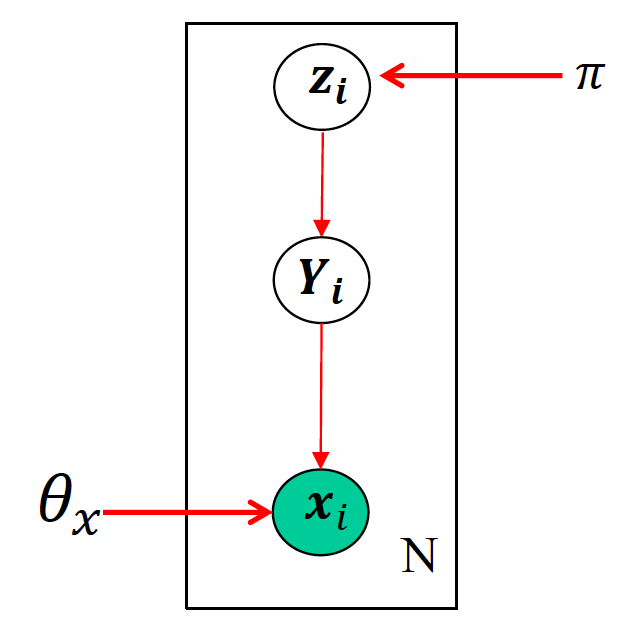
\includegraphics[width = 0.4\hsize]{./figures/PPCAMixture.png} % this includes the figure and specifies that it should span 0.7 times the horizontal size of the 
\caption{Gaussian Mixture Model.} % caption of the figure
\label{fig:PPCA Mixture Model} % a label. When we refer to this label from the text, the figure number is included automatically
\end{center}
\end{figure}




\end{document}
%%% Local Variables: 
%%% mode: latex
%%% TeX-master: t
%%% End: 
